% LaTeX report template 
%

% This is a comment: in LaTeX everything that in a line comes
% after a "%" symbol is treated as comment

\documentclass[11pt, a4paper]{article}
\usepackage{graphicx}
\usepackage{amsmath}
\usepackage{listings}


\title{Assignment 4} % Title

\author{Om Shri Prasath (EE17B113)} % Author name

\date{\today} % Date for the report
\begin{document}	
	
\maketitle % Insert the title, author and date		
	\section{Introduction}
	The report discusses 7 tasks in Python to find Fourier Approximations of two function $e^{x}$ and $\cos(\cos(x))$ from its integral definition and using Least Squares method.\\
	We will fit two functions, $e^{x}$ and $\cos(\cos(x))$ over the interval [0,2$\pi$) using the fourier series
 	\begin{equation}
    a_{0} + \sum\limits_{n=1}^{\infty} {{a_{n}\cos(nx_{i})+b_{n}\sin(nx_{i})}} \approx f(x_{i}) 
    \end{equation}
    	The equations used here to find the Fourier coefficients are as follows:
    \begin{equation}
         a_{0} = \frac{1}{2\pi}\int\limits_{0}^{2\pi} f(x)dx 
    \end{equation}
    \begin{equation}
         a_{n} = \frac{1}{\pi}\int\limits_{0}^{2\pi} f(x)\cos(nx)dx 
    \end{equation}
    \begin{equation}
         b_{n} = \frac{1}{\pi}\int\limits_{0}^{2\pi} f(x)\sin(nx)dx 
    \end{equation}
     \section{Python code}
     
     \begin{lstlisting}

     \end{lstlisting}
     \begin{lstlisting}
# Importing libraries
from pylab import *
from scipy.integrate import quad
     \end{lstlisting}
     \break
     \subsection{Question 1}\label{question-1}

     \begin{itemize}
     \item
       Define Python functions for the two functions \(e^{x}\) and
       \(\cos(\cos(x))\) which return a vector (or scalar) value.\\
     \item
       Plot the functions over the interval {[}−2\(\pi\),\(4\pi\)).
     \item
       Discuss periodicity of both functions
     \item
       Plot the expected functions from fourier series
     \end{itemize}
     \textit{\textbf{Code:}}

     \begin{lstlisting}
def exp_fn(x):
     return exp(x)

def coscos_fn(x):
     return cos(cos(x))

x = linspace(-2*pi, 4*pi, 400)

period = 2*pi

semilogy(x, exp_fn(x), 'k', label="Original Function")

semilogy(x, exp_fn(x % period), '--',
     label="Expected Function from fourier series")
legend()
title(r"Figure 1 : Plot of $e^{x}$")
xlabel(r"x")
ylabel(r"$e^{x}$")
grid()
show()

plot(x, coscos_fn(x), 'b', linewidth=4, label="Original Function")
plot(x, coscos_fn(x % period), 'y--',
     label="Expected Function from fourier series")
legend(loc='upper right')
title(r"Figure 2 : Plot of $\cos(\cos(x))$")
xlabel(r"x")
ylabel(r"$\cos(\cos(x))$")
grid()
show()
     \end{lstlisting}
     \begin{figure}[!tbh]
      \centering
      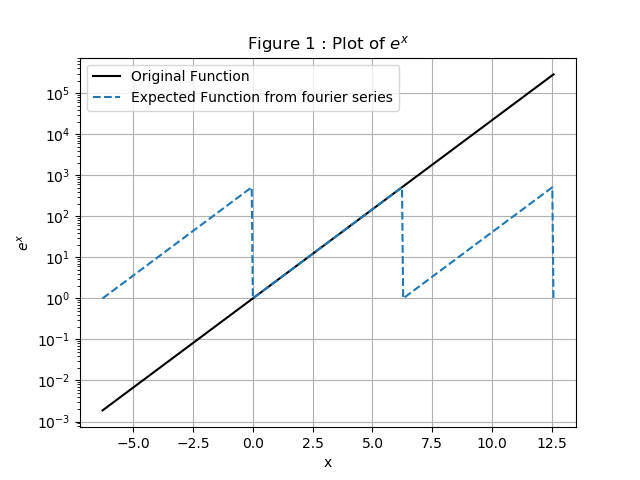
\includegraphics[scale=0.7]{./../Extras/1.png}  % Mention the image name within the curly braces. Image should be in the same folder as the tex file. 
      
      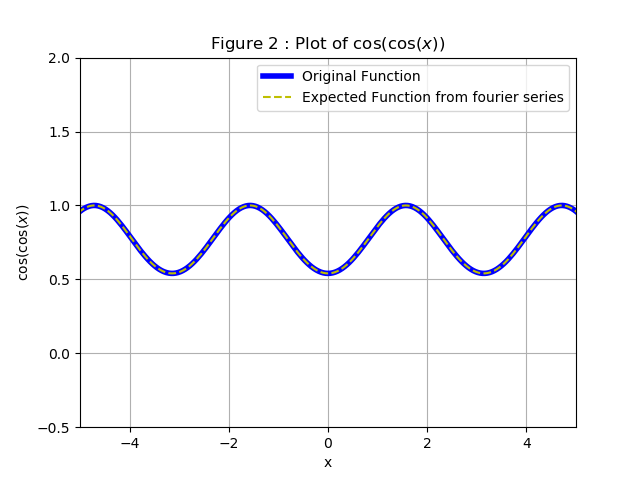
\includegraphics[scale=0.7]{./../Extras/2.png}  % Mention the image name within the curly braces. Image should be in the same folder as the tex file. 
      \caption{Plot for $e^x$ and $cos(cos(x))$}
    \end{figure}
     \break\break
     \subsubsection{Results and Discussion :}\label{results-and-discussion}
     \begin{itemize}
     \item
       We observe that \(e^{x}\) is not periodic, whereas \(\cos(\cos(x))\)
       is periodic as the expected and original function matched for the
       latter but not for \(e^{x}\).
     \item
       Period of \(\cos(\cos(x))\) is \(2\pi\) as we observe from graph and
       \(e^{x}\) monotously increasing hence not periodic.
     \item
       We get expected function by:
     
       \begin{itemize}
       \item
         plotting expected function by dividing the x by period and giving
         remainder as input to the function, so that x values repeat after
         given period.
       \item
         That is f(x\%period) is now the expected periodic function from
         fourier series.
       \end{itemize}
     \end{itemize}
     \break
     \subsection{Question 2}\label{question-2}

     \begin{itemize}
     \item
       Obtain the first 51 coefficients i.e \(a_{0}, a_{1}, b_{1},....\) for
       \(e^{x}\) and \(\cos(\cos(x))\) using scipy quad function
     \item
       And to calculate the function using those coefficients and comparing
       with original funcitons graphically.
     \end{itemize}
     
     \textit{\textbf{Code:}}
     \begin{lstlisting}

def an_fourier(x, k, f):
     return f(x)*cos(k*x)


def bn_fourier(x, k, f):
     return f(x)*sin(k*x)

def find_coeff(f):

     coeff = []
     coeff.append((quad(f, 0, 2*pi)[0])/(2*pi))
     for i in range(1, 26):
     coeff.append((quad(an_fourier, 0, 2*pi, args=(i, f))[0])/pi)
     coeff.append((quad(bn_fourier, 0, 2*pi, args=(i, f))[0])/pi)
     return coeff

def matrix_create(nrow, ncol, x):
     A = zeros((nrow, ncol))  # allocate space for A
     A[:, 0] = 1  # col 1 is all ones
     for k in range(1, int((ncol+1)/2)):
     A[:, 2*k-1] = cos(k*x)  # cos(kx) column
     A[:, 2*k] = sin(k*x)  # sin(kx) column
     # endfor
     return A

def compute_fn(c):
     A = matrix_create(400, 51, x)
     f_fourier = A.dot(c)
     return f_fourier


exp_coeff = []
coscos_coeff = []
exp_coeff1 = []
coscos_coeff1 = []

exp_coeff1 = find_coeff(exp_fn)
coscos_coeff1 = find_coeff(coscos_fn)

exp_coeff = np.abs(exp_coeff1)
coscos_coeff = np.abs(coscos_coeff1)

exp_fn_fourier = compute_fn(exp_coeff1)
coscos_fn_fourier = compute_fn(coscos_coeff1)


semilogy(x, exp_fn_fourier, 'ro', label="Function using Fourier Coefficients")
ylim([pow(10, -1), pow(10, 4)])
legend()

grid()
show()


plot(x, coscos_fn_fourier, 'ro', label="Function using Fourier Coefficients")
legend(loc='upper right')

grid()
show()
     \end{lstlisting}
     \break
     \begin{figure}[!tbh]
          \centering
          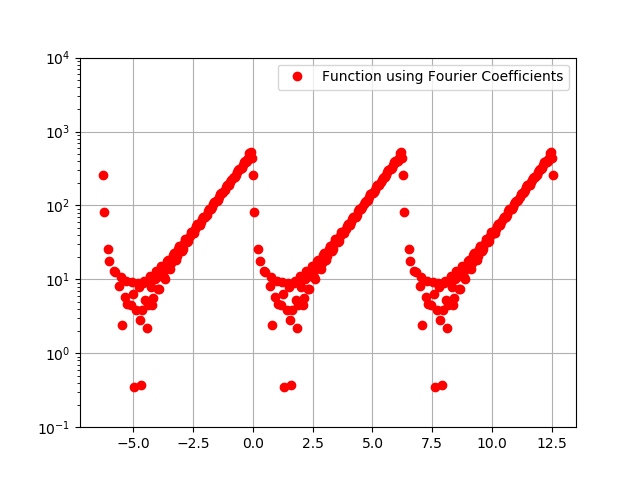
\includegraphics[scale=0.8]{./../Extras/3.png}  
          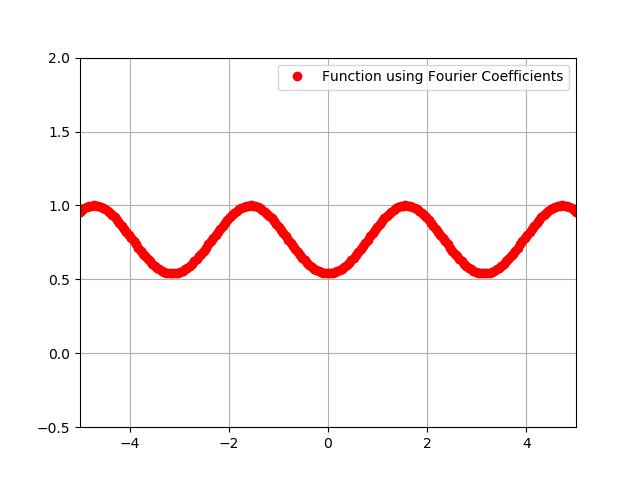
\includegraphics[scale=0.8]{./../Extras/4.png}  
          \caption{Plot for Fourier Appriximation of $e^x$ and $cos(cos(x))$}
     \end{figure}
     \break

    \subsection{Question3}\label{question3}

    \begin{itemize}
    \item
      Two different plots for each function using ``semilogy'' and
      ``loglog'' and plot the magnitude of the coefficients vs n
    \item
      And to analyse them and to discuss the observations. \#\# Plots:
    \item
      For each function magnitude of \(a_{n}\) and \(b_{n}\) coefficients
      which are computed using integration are plotted in same figure in
      semilog as well as loglog plot for simpler comparisons.
    \end{itemize}

    \textit{\textbf{Code:}}
    \begin{lstlisting}
semilogy((exp_coeff[1::2]), 'ro', label=r"$a_{n}$ using Integration")
semilogy((exp_coeff[2::2]), 'ko', label=r"$b_{n}$ using Integration")
legend()
title("Figure 3 : Fourier coefficients of $e^{x}$ (semi-log)")
xlabel("n")
ylabel("Magnitude of coeffients")

grid()
show()

loglog((exp_coeff[1::2]), 'ro', label=r"$a_{n}$ using Integration")
loglog((exp_coeff[2::2]), 'ko', label=r"$b_{n}$ using Integration")
legend(loc='upper right')
title("Figure 4 : Fourier coefficients of $e^{x}$ (Log-Log)")
xlabel("n")

grid()
ylabel("Magnitude of coeffients")
show()

semilogy((coscos_coeff[1::2]), 'ro', label=r"$a_{n}$ using Integration")
semilogy((coscos_coeff[2::2]), 'ko', label=r"$b_{n}$ using Integration")
legend(loc='upper right')
title("Figure 5 : Fourier coefficients of $\cos(\cos(x))$ (semi-log)")
xlabel("n")

grid()
ylabel("Magnitude of coeffients")
show()

loglog((coscos_coeff[1::2]), 'ro', label=r"$a_{n}$ using Integration")
loglog((coscos_coeff[2::2]), 'ko', label=r"$b_{n}$ using Integration")
legend(loc='upper right')
title("Figure 6 : Fourier coefficients of $\cos(\cos(x))$  (Log-Log)")
xlabel("n")

grid()
ylabel("Magnitude of coeffients")
show()

    \end{lstlisting}
  \begin{figure}[!tbh]
     \centering
     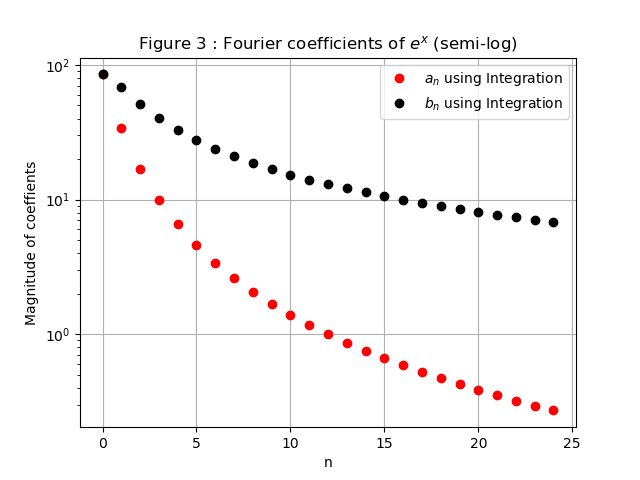
\includegraphics[scale=0.75]{./../Extras/5.png}  
     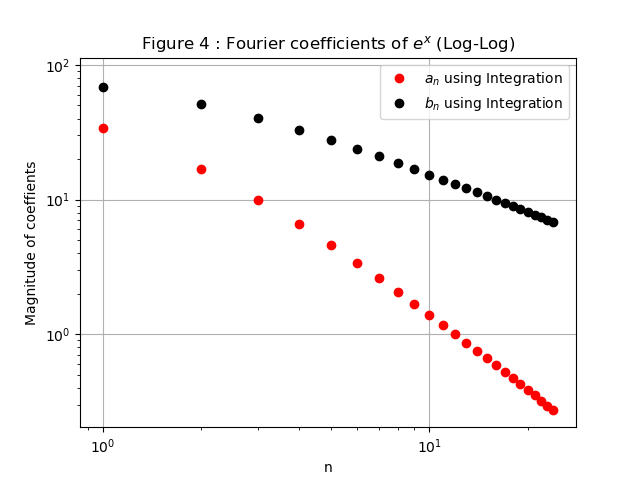
\includegraphics[scale=0.75]{./../Extras/6.png}
     \caption{Semi-Log ,Log-Log plots of Fourier coefficients of $e^x$ (Integration)}  
\end{figure}
\begin{figure}[!tbh]
     \centering
     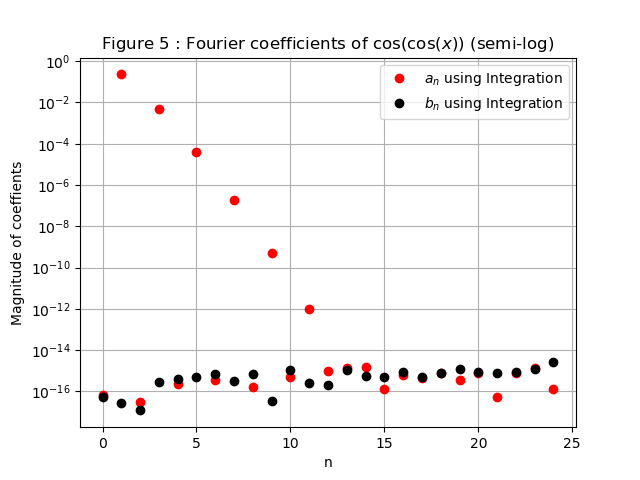
\includegraphics[scale=0.8]{./../Extras/7.png}  
     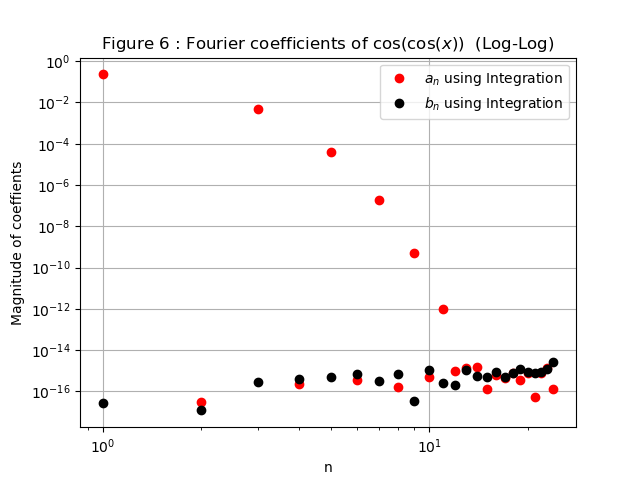
\includegraphics[scale=0.8]{./../Extras/8.png}  
     \caption{Semi-Log ,Log-Log plots of Fourier coefficients of $cos(cos(x))$ (Integration)}
\end{figure}
\clearpage
\subsubsection{Results and Observations :}\label{results-and-observations}
\begin{itemize}
     \item
       The \(b_{n}\) coefficients in the second case should be nearly zero.
       Why does this happen?
       \begin{itemize}
          \item
       Because \(\cos(\cos(x))\) is an even function and for finding
       \(b_{n}\) we use Eq.(4) so the whole integral can be integrated in any
       interval with length of \(2\pi\), so for convenience we choose
       \([-\pi,\pi)\) , then the integrand is odd since \(\sin(nx)\) is
       there. so the integral becomes zero analytically. Where as here we
       compute using quad function which uses numerical methods so \(b_{n}\)
       is very small but not exactly zero.
       \end{itemize}
     \item
       In the first case, the coefficients do not decay as quickly as the
       coefficients for the second case. Why not?
          \begin{itemize}
          \item
       Rate of decay of fourier coefficients is determined by how smooth the
       function is,if a function is infinitely differentiable then its
       fourier coefficients decays very faster, where as if \(k^{th}\)
       derivative of function is discontinous the coefficients falls as
       \(\frac{1}{n^{k+1}}\). to atleast converge.So in first case i.e is
       \(e^{x}\) is not periodic hence discontinous at \(2n\pi\) so the
       function itself is discontinous so coefficients falls as
       \(\frac{1}{n}\) so we need more coefficients for more
       accuracy,coefficients doesn't decay as quickly as for
       \(\cos(\cos(x))\) as it is infinitely differentiable and smooth so we
       need less no of coefficients to reconstruct the function so it decays
       faster.
     \end{itemize}		
          
     \item
       Why does loglog plot in Figure 4 look linear, wheras the semilog plot
       in Figure 5 looks linear?
       \begin{itemize}
       \item
       Because the coefficients of \(e^{x}\) varies as \(n^{k}\) where as
       \(\cos(\cos(x))\) varies exponentially with 'n' means \(\alpha^{n}\) ,
       thats why loglog looks linear in first case and semilog in second
       case.
     \end{itemize}
       \end{itemize}
     \break
       \subsection{Question 4 \& 5}\label{question-4-5}

       \begin{itemize}
       \item
         Uses least squares method approach to find the fourier coefficients of
         \(e^{x}\) and \(\cos(\cos(x))\)
       \item
         Evaluate both the functions at each x values and call it b. Now this
         is approximated by
         \(a_{0} + \sum\limits_{n=1}^{\infty} {{a_{n}\cos(nx)+b_{n}\sin(nx)}}\)
       \item
         such that
       
         \begin{equation}
         a_{0} + \sum\limits_{n=1}^{\infty} {{a_{n}\cos(nx_{i})+b_{n}\sin(nx_{i})}} \approx f(x_{i}) 
         \end{equation}
       \item
         To implement this we use matrices to find the coefficients using Least
         Squares method using inbuilt python function 'lstsq'
       \end{itemize}

    \textit{\textbf{Code:}}
    \begin{lstlisting}

def lstsq_coeff(f, low_lim, upp_lim, no_points):
     x1 = linspace(low_lim, upp_lim, no_points)
     # drop last term to have a proper periodic integral
     x1 = x1[:-1]
     b = []
     b = f(x1)
     A = matrix_create(no_points-1, 51, x1)
     c = []
     c = lstsq(A, b, rcond=None)[0] 

     return c

coeff_exp = lstsq_coeff(exp_fn, 0, 2*pi, 401)
coeff_coscos = lstsq_coeff(coscos_fn, 0, 2*pi, 401)

c1 = np.abs(coeff_exp)
c2 = np.abs(coeff_coscos)

semilogy((c1[1::2]), 'go', label=r"$a_{n}$ using Least Squares")
semilogy((c1[2::2]), 'bo', label=r"$b_{n}$ using Least Squares")

grid()
legend(loc='upper right')
show()


loglog((c1[1::2]), 'go', label=r"$a_{n}$ using Least Squares ")
loglog((c1[2::2]), 'bo', label=r"$b_{n}$ using Least Squares")

grid()
legend(loc='lower left')
show()


semilogy((c2[1::2]), 'go', label=r"$a_{n}$ using Least Squares")
semilogy((c2[2::2]), 'bo', label=r"$b_{n}$ using Least Squares")


grid()
legend(loc='upper right')
show()

loglog((c2[1::2]), 'go', label=r"$a_{n}$ using Least Squares ")
loglog((c2[2::2]), 'bo', label=r"$b_{n}$ using Least Squares")

grid()
legend(loc=0)
show()
    \end{lstlisting}
\break
\begin{figure}[!tbh]
     \centering
     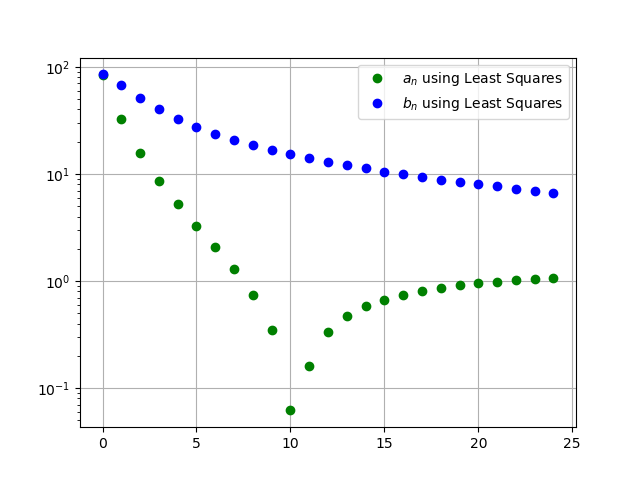
\includegraphics[scale=0.7]{./../Extras/9.png}  
     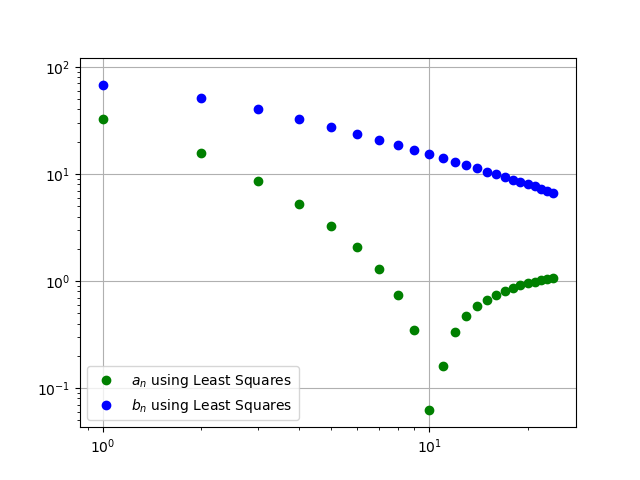
\includegraphics[scale=0.7]{./../Extras/10.png}  
     \caption{Semi-Log ,Log-Log plots of coefficients of $e^x$(Least Squares)}  
\end{figure}
\begin{figure}[!tbh]
     \centering
     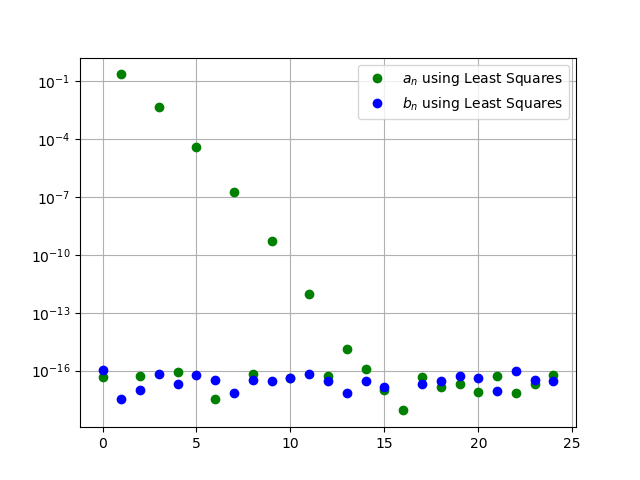
\includegraphics[scale=0.7]{./../Extras/11.png}  
     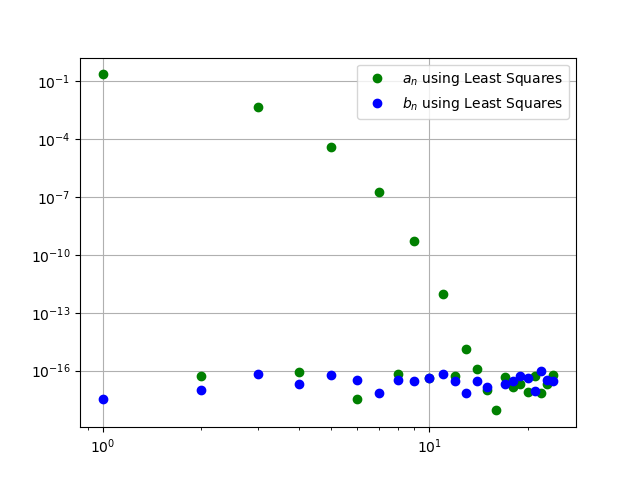
\includegraphics[scale=0.7]{./../Extras/12.png}  
     \caption{Semi-Log ,Log-Log plots of coefficients of $cos(cos(x))$(Least Squares)}  
\end{figure}
\clearpage
\subsection{Question 6}\label{question-6}

\begin{itemize}
\item
  To compare the answers got by least squares and by the direct
  integration.
\item
  And finding deviation between them and find the largest deviation
  using Vectors
\end{itemize}

\textit{\textbf{Code:}}
\begin{lstlisting}

def coeff_compare(f):
    deviations = []
    max_dev = 0
    if(f == 1):
        deviations = np.abs(exp_coeff1 - coeff_exp)
    elif(f == 2):
        deviations = np.abs(coscos_coeff1 - coeff_coscos)

    max_dev = np.amax(deviations)
    return deviations, max_dev


dev1, maxdev1 = coeff_compare(1)
dev2, maxdev2 = coeff_compare(2)

print("Maximum deviation in exp coefficients : ", maxdev1)
print("Maximum deviation in cos_cos coefficients : ", maxdev2)
plot(dev1, 'g')
title(r"Figure 7 : Deviation between Coefficients for $e^{x}$")
grid()
xlabel("n")
ylabel("Magnitude of Deviations")
show()

plot(dev2, 'g')
title(r"Figure 8 : Deviation between coefficients for $\cos(\cos(x))$")
grid()
xlabel("n")
ylabel("Magnitude of Deviations")
show()

\end{lstlisting}
\break

\begin{figure}[!tbh]
     \centering
     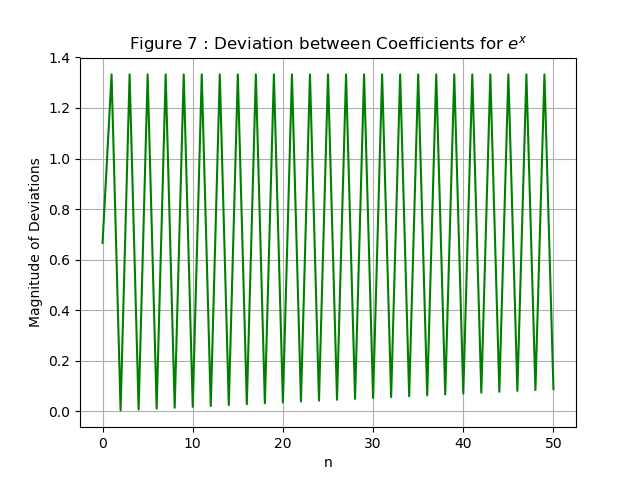
\includegraphics[scale=0.7]{./../Extras/13.png}  
     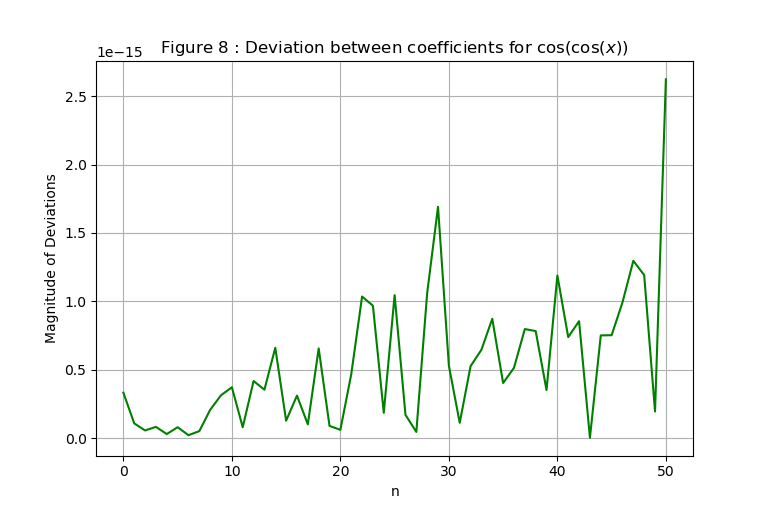
\includegraphics[scale=0.6]{./../Extras/14.png}  
     \caption{Deviation plots of Fourier coefficients of both the functions found via integration and least-squares}
\end{figure}
\break
\subsubsection{Results and Discussion :}\label{results-and-discussion}
\begin{itemize}
  \item 
  The maximum deviation for :
    \begin{itemize}
      \item exp(x) = 1.3327308703353111
      \item cos(cos(x)) = 2.622704669603838e-15
    \end{itemize}
  \end{itemize}
\break
\subsection{Question 7}\label{question-7}

\begin{itemize}
\item
  Computing Ac i.e multiplying Matrix A and Vector C from the estimated
  values of Coeffient Vector C by Least Squares Method.
\item
  To Plot them (with green circles) in Figures 1 and 2 respectively for
  the two functions.
  
\end{itemize}

\textit{\textbf{Code:}}
\begin{lstlisting}
x1 = linspace(0, 2*pi, 400)

def fn_create_lstsq(c):
     f_lstsq = []
     A = matrix_create(400, 51, x1)
     f_lstsq = A.dot(c)
     return f_lstsq


exp_fn_lstsq = fn_create_lstsq(coeff_exp)
coscos_fn_lstsq = fn_create_lstsq(coeff_coscos)

semilogy(x1, exp_fn_lstsq, 'go',
          label="Inverse Fourier Transform From Least Squares")
legend()

grid()
ylim([pow(10, -2), pow(10, 3)])
xlim([0, 2*pi])
show()

plot(x1, coscos_fn_lstsq, 'go', markersize=4,
     label="Inverse Fourier Transform From Least Squares")
ylim([0.5, 1.3])
xlim([0, 2*pi])
grid()
legend()
show()
     
\end{lstlisting}
\break

\begin{figure}[!tbh]
     \centering
     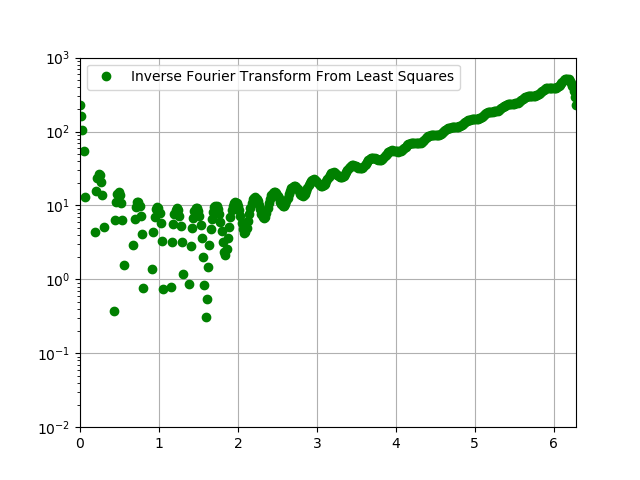
\includegraphics[scale=0.8]{./../Extras/15.png}  
     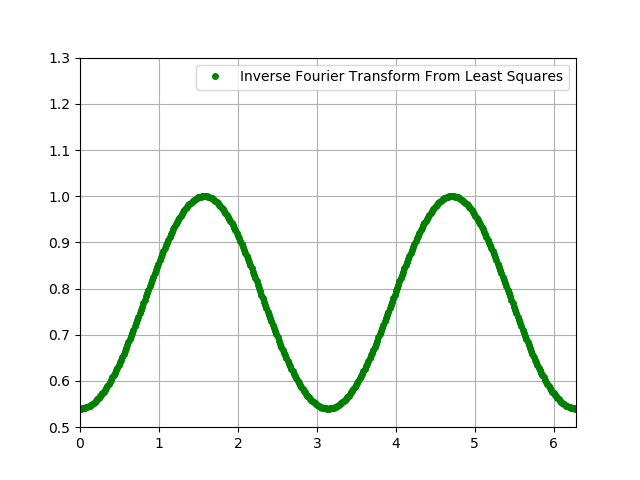
\includegraphics[scale=0.8]{./../Extras/16.png}  
     \caption{Plots of the functions got by Inverse Fourier Transform}
\end{figure}
\subsubsection{Results and Discussion :}\label{results-and-discussion}

\begin{itemize}

\item
  As we observe that there is a significant deviation for \(e^{x}\) as
  it has discontinuites at \(2n\pi\) which can be observed in Figure 1
  and so there will be \textbf{Gibbs phenomenon} i.e there will be
  oscillations around the discontinuity points and their ripple
  amplitude will decrease as we go close to discontinuity. In this case
  it is at \(2\pi\) for \(e^{x}\).
\item
  As we observe that rimples are high in starting and reduces and
  oscillate with more frequency as we go towards \(2\pi\). This
  phenomenon is called \textbf{Gibbs Phenomenon}
\item
  Due to this. the orginal function and one which is reconstructed using
  least squares will not fit exactly.
\item
  And as we know that Fourier series is used to define periodic signals
  in frequency domain and \(e^{x}\) is a aperiodic signal so you can't
  define an aperiodic signal on an interval of finite length (if you
  try, you'll lose information about the signal), so one must use the
  Fourier transform for such a signal.
\item
  Thats why there are significant deviations for \(e^{x}\) from original
  function.
\item
  Whereas for \(\cos(\cos(x))\) the curves fit almost perfectly because
  the function itself is a periodic function and it is a continous
  function in entire x range so we get very negligible deviation and
  able to reconstruct the signal with just the fourier coefficients.
\end{itemize}
\section{Conclusion}
We see that the fourier estimation of \(e^x\) does not match
significantly with the function close to \(0\), but matches near
perfectly in the case of \(\cos(\cos(x))\). This is due to the
presence of a discontiuity at \(x=0\) for the periodic extension of
\(e^x\). This discontiuity leads to non-uniform convergence of the
fourier series, with different rates for both the functions.\\\\
The difference in the rates of convergence leads to the \textbf{Gibb's
phenomenon}, which is the ringing observed at discontiuities in the
fourier estimation of a discontiuous function. 
This explains the mismatch in the fourier approximation for \(e^x\).
\\\\
Thus we can conclude that the Fourier Series Approximation Method works extremely well
for smooth periodic functions, but gives bad results for discontinuos periodic functions
\end{document}